\section{Darbības princips} \label{section:mechanism}
% fotons uzspīd elektronam un viņu ierosina un tad tas aiziet pāri vadītspējas zonai un aizpeld uz elektrodu un caurums aizpeld uz otru elektrodu un rodas potenciālu starpība no kurienes strāva.

Saules paneļi sastāv no fotoelementiem, kas pārveido gaismas enerģiju elektriskā lauka enerģijā. Fotoelements, kura uzbūves shēma ir parādīta \ref{fig:PV}. attēlā, ir p-n pāreja ar elektriskajiem kontaktiem, kas pieslēgti pie lādētāja vai cita enerģijas patērētāja. Fotoelementa apakšējā daļa sastāv no n-tipa pusvadītāja, kurā lādiņa pamatnesēji ir elektroni, bet augšējā daļa -- no p-tipa pusvadītāja, kur lādiņa pamatnesēji ir caurumi. 

\begin{figure}[h]
    \centering
    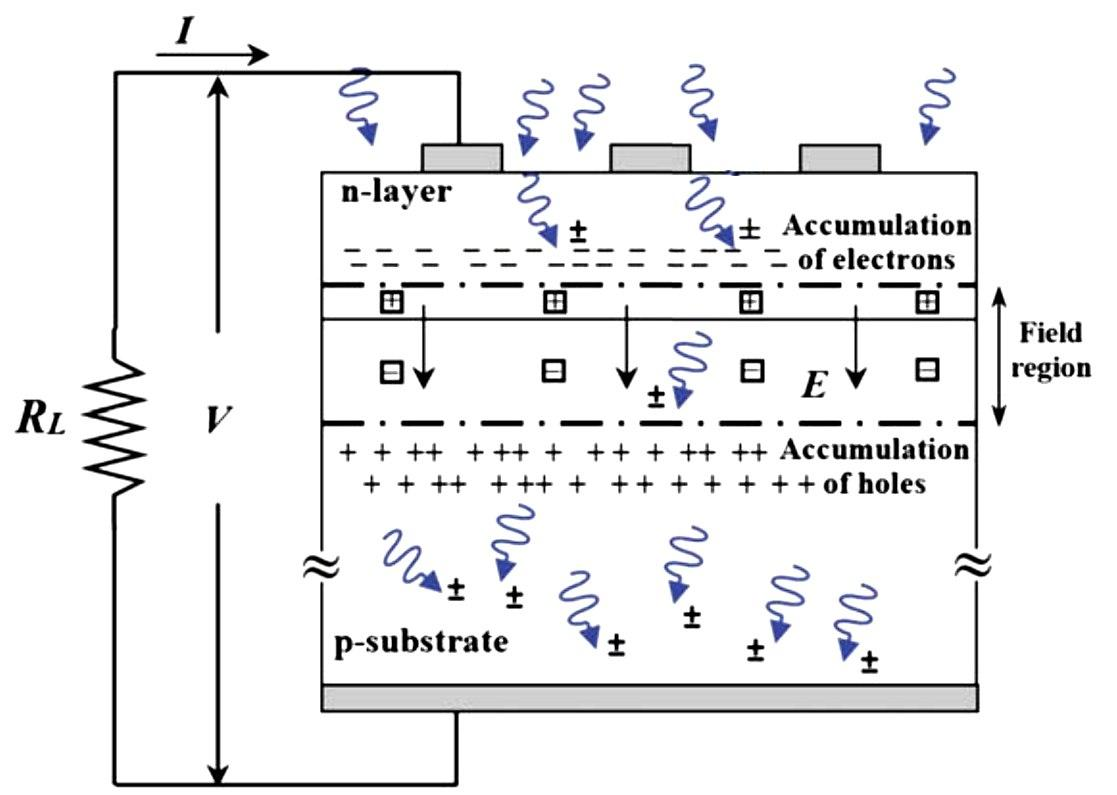
\includegraphics[width=0.6\linewidth]{figures/misc/PV.jpg}
    \caption{Saules paneļa shēma. Tas sastāv no fotoelementiem, kuru augšējais slānis veidots no p-tipa pusvadītāja, bet apakšējais --- no n-tipa pusvadītāja~\cite{Yahyaoui}.}
    \label{fig:PV}
\end{figure}

P-tipa un n-tipa pusvadītāja īpašības var panākt, piemēram, dopējot silīcija kristālu ar attiecīgi III vai V grupas elementiem. Ja silīcija kristālam pievieno bora atomus nelielā koncentrācijā, izveidojas \ref{fig:p-n-type}. att. pa kreisi redzamā situācija. Katram Si atomam ir četri elektroni ārējā čaulā, ar kuru palīdzību atoms izveido četras kovalentās saites ar četriem citiem atomiem. Savukārt bors, būdams III grupas elements, var izveidot tikai trīs saites. Tādā veidā pie bora atoma parādās "caurums" -- nenoslēgta kovalentā saite, kas attēlā apzīmēta ar sarkanu apli. Uz šo vietu var pārvietoties kāds no blakus esošiem elektroniem, bet tad neaizpildīta vieta parādīsies pie blakus esošā atoma. Tādā veidā var uzskatīt, ka caurums pārvietojas, un nosaukt to par pozitīvo lādiņa nesēju. Šādus pusvadītājus sauc par p-tipa pusvadītājiem. ~\cite{Yahyaoui}

Ja silīcija kristālam pievieno fosfora atomus, izveidojas pretēja situācija -- pie P atoma parādās elektrons, kas nepiedalās saites veidošanā (sk. att. \ref{fig:p-n-type}., pa labi). Lai pārvietotos, brīvajam elektronam ir nepieciešams mazāk enerģijas nekā elektroniem, kas veido kovalentās saites starp Si atomiem. Tātad, lādiņa pamatnesēji n-tipa pusvadītājos ir elektroni.

Dopējot divus blakus esošus Si kristāla apgabalus dažādā veidā, iegūst p-n pāreju. Uz robežas starp apgabaliem elektroni no n-tipa apgabala var rekombinēties jeb difūzijas ceļā nokļūt uz p-tipa apgabalu un aizpildīt pietiekami tuvu esošus caurumus, tāpēc p-tipa pusvadītājā mala uzlādējas negatīvi.

\begin{figure}[h]
	\centering
	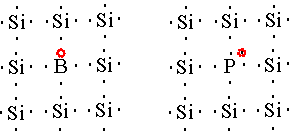
\includegraphics[width=0.5\linewidth]{figures/misc/p_n_type.pdf}
	\caption{Silīcija kristāla 2D izklājums, atomu ārējās čaulas elektroni ir apzīmēti ar punktiem. Pievienojot bora atomu, iegūst p-tipa pusvadītāju (pa kreisi), bet fosfora atomu --- n-tipa pusvadītāju (pa labi).}
	\label{fig:p-n-type}
\end{figure}

Fotoelementa darbība balstās uz iekšējo fotoelektrisko efektu -- parādību, kad elektrons tiek ierosināts ar gaismas kvantu un pāriet no valences zonas uz vadītspējas zonu. Kad tas notiek augšējā slānī (p-tipa pusvadītājā), elektrons atgrūžas no robežas starp slāņiem, kura ir negatīvi lādēta rekombinācijas dēļ. Negatīvi lādētā (no p-tipa pusvadītāja puses) robeža rada potenciālu starpību, kas veicina elektronu kustību pa vadiem uz patērētāju, tādā veidā radot elektrisko strāvu.